\section{Evaluation Framework}
\label{sec:eval_frameworks}
% \KZ{Are we only evaluating the final version of the two bots from prev section? This is not part of the iterative design process right? This should be made clearer.}
% \MY{normally we provide objective/automatic eva first, followed by human evaluation results. when introducing the metrics and results, follow this order}

Guided by psychiatrists and through an iterative development process, we established the objectives for two chatbots and completed their designs in Phase 2. In addition, we also designed an evaluation framework, which will be employed in Phase 3 to assess the performance of the developed chatbots. This section will describe our evaluation framework which encompasses interactive experiments for human evaluation and various task-specific metrics.
\subsection{Chatbots of Comparison}
% \KZ{this section should go into the evaluation framework?}

Due to the complexity and high time cost of human evaluation, we select several representative prompt versions for comparison, and discuss the evaluation process of doctor and patient chatbots respectively.

\paragraph{Doctor Chatbot} 
Each patient will have a conversation with four different doctor chatbots in a random order, and then rate them on four human evaluation metrics with 1-4 scale. 
Three of the chatbots are powered by ChatGPT. \texttt{D1} uses the full prompt, 
while the other two (i.e., \texttt{D2}, 
\texttt{D3}) have certain parts removed for ablation. 
The fourth chatbot, \texttt{CPT}, is a representative deep learning chatbot trained on domain-specific data \cite{yao-etal-2022-d4} using CPT model~\cite{shao2021cpt}. 
% \MY{Make a table for these bots, including doctor and patient}
\paragraph{Patient Chatbot}
Each psychiatrist will have a conversation with two patient chatbots, and then rate their performance with 1-4 scale. 
The two patient chatbots are \texttt{P1} and \texttt{P2}, aligning with the prompt versions in Section \ref{sec:pat_prompt}. 
A brief description of these chatbots can be found in Table \ref{tab:cmp_chatbots}.
% The first one uses the full prompt while the second one omits additional parts for realistic in version 2\footnote{Detailed description and prompt of these doctor/patient chatbots are shown in Appendix \ref{apd:prompts}.}.
% COMMENT: 这两段要引述一下表1啊。此外1中的"xx parts"的表述,最好和前面一致,都用v1v2v3或者①②③这种方式来提,更容易理解。CPT这个模型的名字也应该在正文里写出来。

\begin{table}[h]
    \centering
    \footnotesize
    \begin{tabular}{m{0.1\columnwidth}|c|m{0.6\columnwidth}}
    \hline
    & Chatbot & Description \\
    \hline
    \multirow{4}{0.1\columnwidth}{Doctor} & D1 & use the full doctor prompt \\
    \cline{2-3}
    & D2 & remove empathy parts in prompt  \\
    \cline{2-3}
    & D3 &  remove aspect part in prompt \\
    \cline{2-3}
    & CPT & CPT model trained on domain data \\
    \hline
    \multirow{2}{0.1\columnwidth}{Patient} & P1 & use the prompt in the first iteration \\
    \cline{2-3}
    & P2 & use the full patient prompt\\
    \hline
    \end{tabular}
    \caption{Brief description of the chatbots for comparison. Detailed description and prompt is in Appendix \ref{apd:prompts}.}
    \label{tab:cmp_chatbots}
\end{table}
\subsection{Evaluation Metrics}
\label{sec:eval_metric}
When designing evaluation metrics, our goal is to ensure that each objective is accompanied by appropriate metrics for accurate measurement.  We employ both human and automatic metrics for evaluation, and divide the automatic metrics of both kind of chatbots into two types: \textbf{function} and \textbf{style}. The overview of these metrics and their relations to objectives can be found in \figref{fig:all_metric}.
% \MY{Clearer now, but still mixing function and style - which objectives and metrics are function-related and which are style?}.
% NEWCOMMENT: 这里这样分类之后,在图中也要把两类指标区分出来,可以在objective那一列上做区分
\begin{figure}[th]
	\centering
	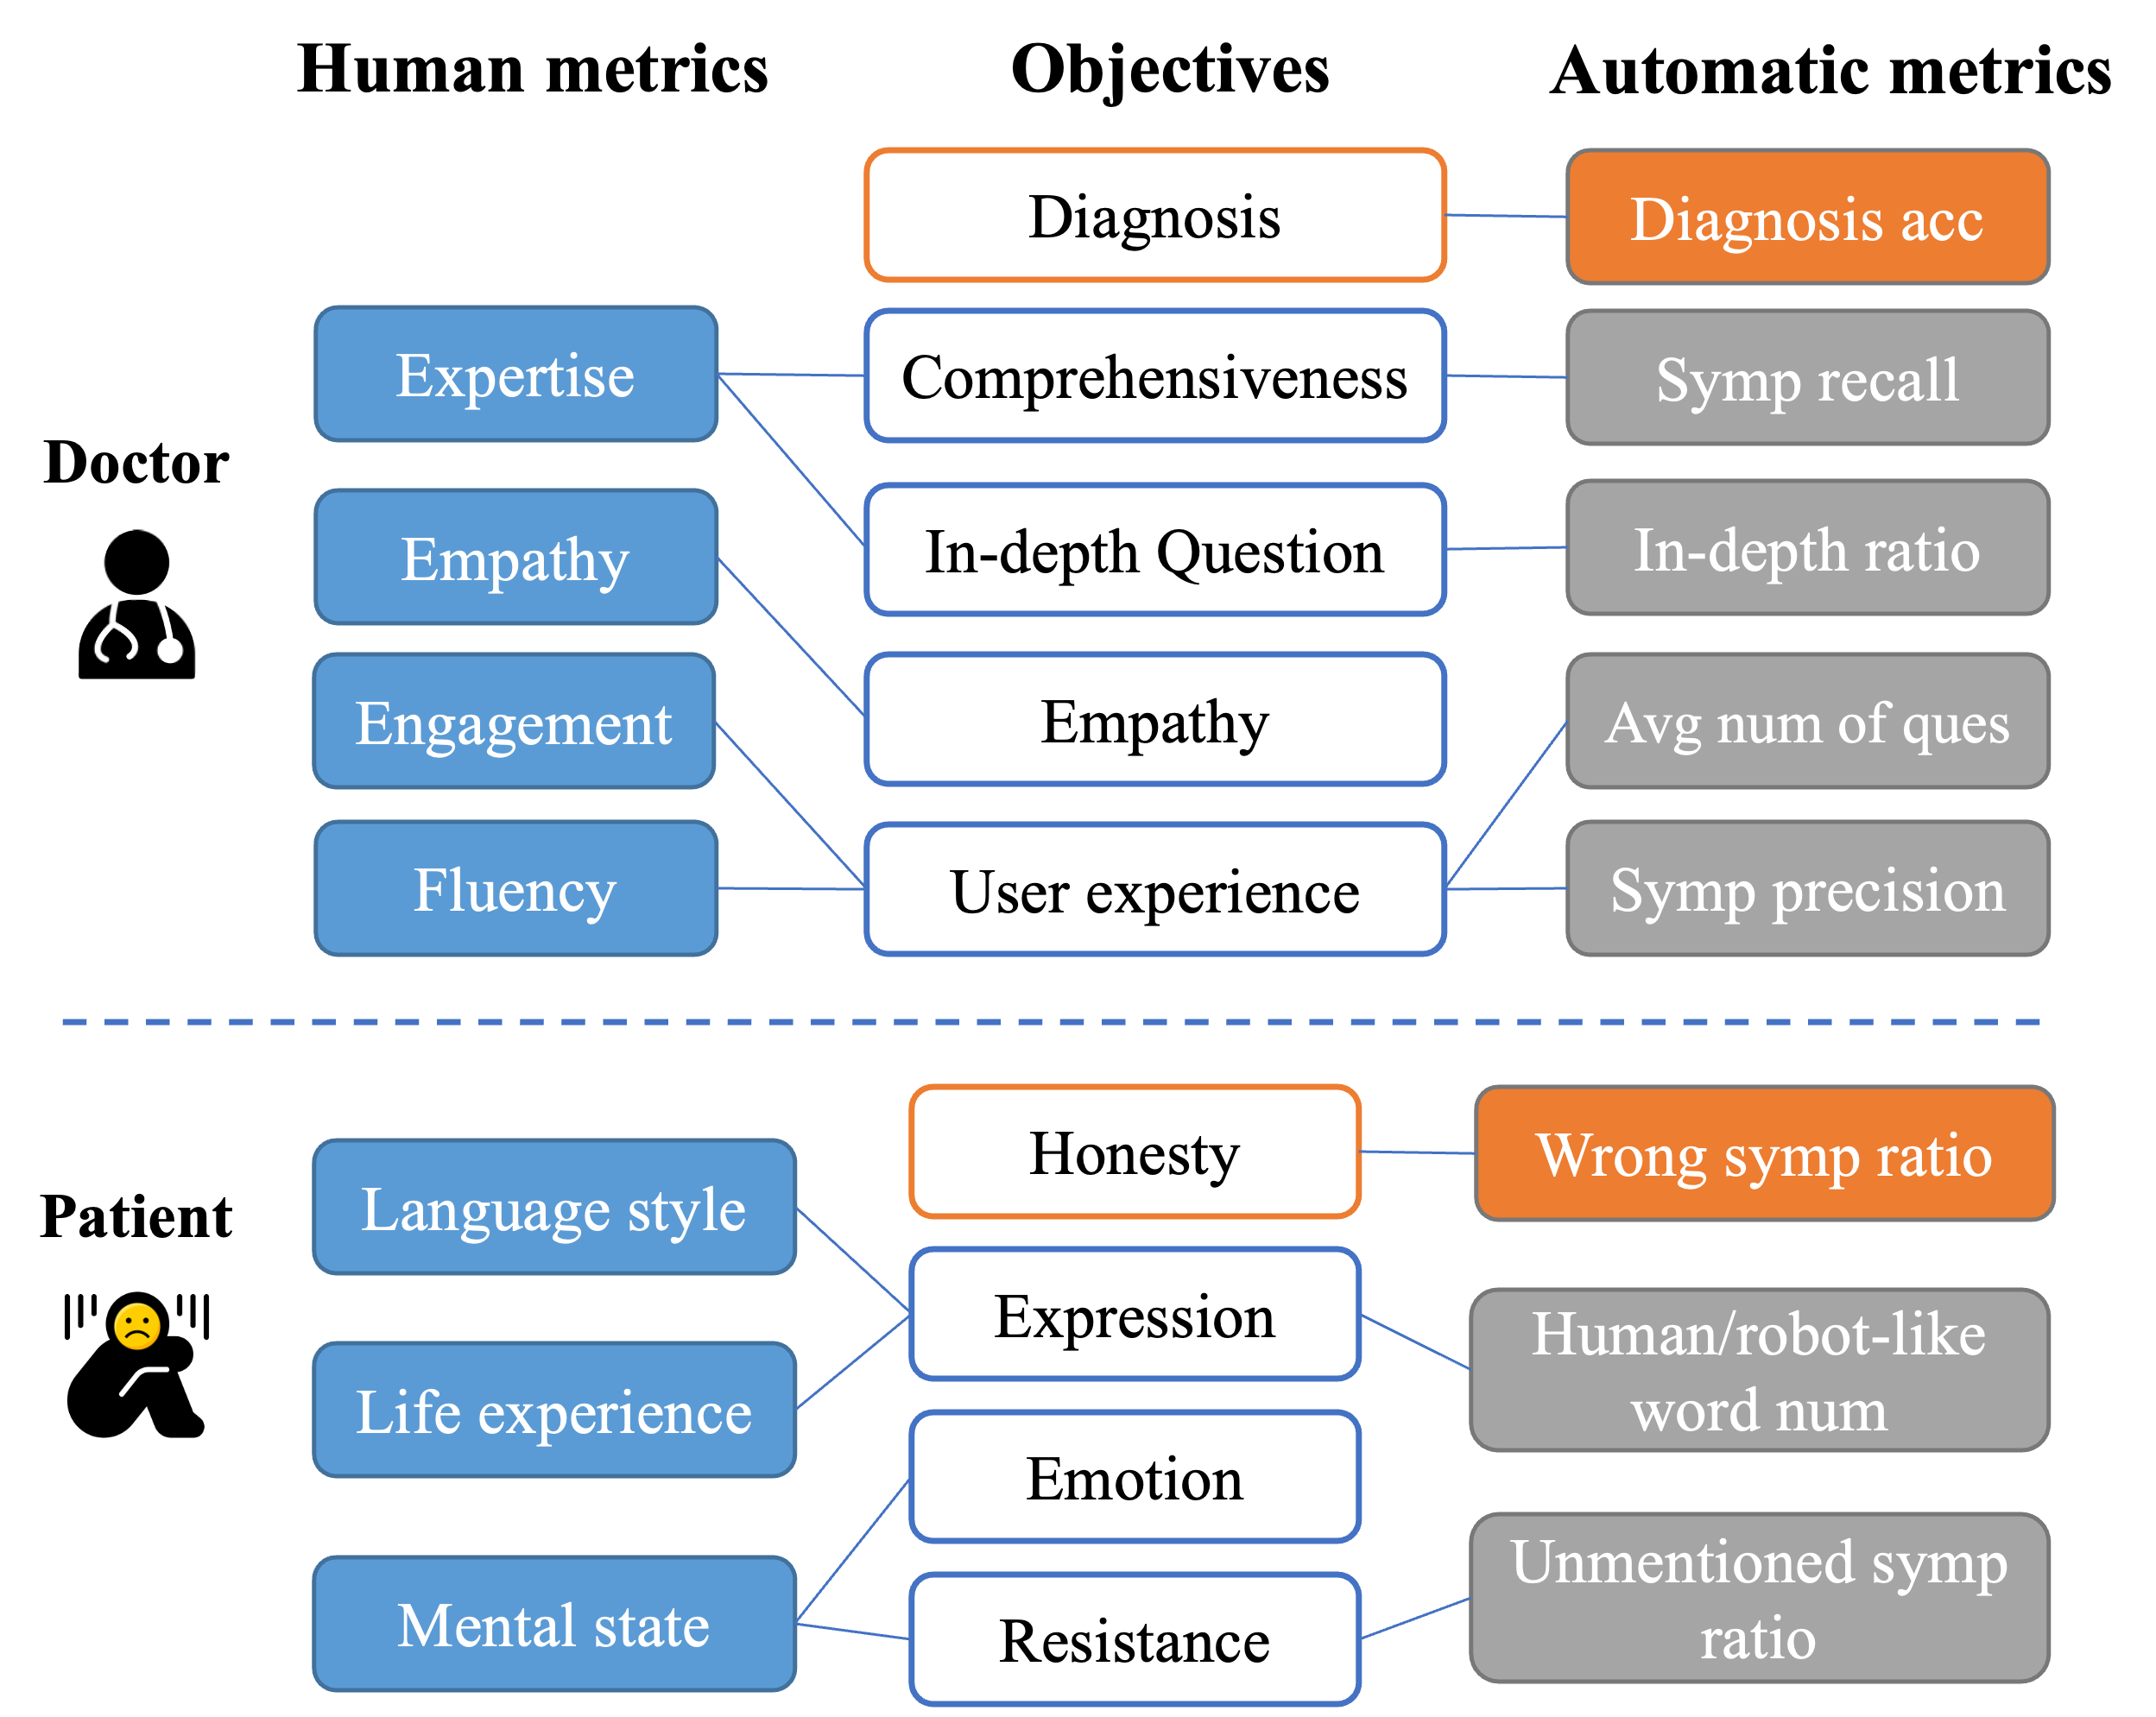
\includegraphics[width=\linewidth]{Figures/metrics.png}
	\caption{The correspondence between evaluation metrics and objectives. \textbf{\textit{Function}} metrics are orange, and \textbf{\textit{style}} metrics are gray.}
	\label{fig:all_metric}
\end{figure}

\subsubsection{Metrics for Doctor Chatbot}
\label{sec:doc_metric}
\paragraph{Human evaluation} In most cases, patients do not have specialized knowledge in psychiatry, making it difficult for them to assess a doctor's professional skills precisely. Therefore, when designing human evaluation metrics for doctor chatbots, we focus mainly on the user experience. The metrics are shown in Table \ref{tab:human_eval_doctor}.
\begin{table}[h]
    \centering
    \footnotesize
    \begin{tabular}{m{0.18\columnwidth}|m{0.7\columnwidth}}
    \hline
    Metrics & Explanation \\
    \hline
    Fluency & The chatbot does not repeat previously asked questions and can smoothly switch between different topics. \\
    \hline
    Empathy & The chatbot can understand and comfort you properly. \\
    \hline
    Expertise & The chatbot behaves like a real doctor, making you believe in its professionalism. \\
    \hline
    Engagement & The chatbot can maintain your attention and make you want to continue talking to it. \\
    \hline
    \end{tabular}
    \caption{Human evaluation metrics of doctor chatbot.}
    \label{tab:human_eval_doctor}
\end{table}
\paragraph{Automatic evaluation}
Different from human evaluation metrics, we mainly measure the expertise of the doctor chatbot using automatic metrics. 
The \textit{functional} requirements for doctor chatbot is to provide an accurate diagnosis, so the corresponding metric is \uline{``diagnosis accuracy''}. 
The \textit{style} part concerns the doctor chatbot's professional skills. We use \uline{``symptom recall''} to evaluate the chatbot's ability to comprehensively gather the patient's symptom-related information, and use \uline{``in-depth ratio''} to assess the ability to ask in-depth questions for deeper understanding. 
To ensure a better user experience, we calculate the \uline{``average number of questions''} asked in a single interaction to discourage the chatbot from overwhelming patients with excessive queries. Furthermore, we employ the metric of \uline{``symptom precision''} to penalize the chatbot's mechanistic behavior of asking all potential questions, irrespective of the user's responses. 

\subsubsection{Metrics for Patient Chatbot}
\label{sec:pat_metric}
\paragraph{Human evaluation}
There is no standard to measure whether a patient is ``good'' enough. Thus, when chatting with patient chatbots, doctors can only assess whether their style of expression and manner of communication resemble real patients enough and whether they can describe their symptoms in a reasonable way, so the main metrics for human evaluation are \textbf{Resemblance} and \textbf{Rationality}.
What's more, we divide the Resemblance metric into three aspects in Table \ref{tab:human_eval_patient}, according to the objectives in Section \ref{sec:objectives}.

\begin{table}[h]
    \centering
    \footnotesize
    \begin{tabular}{m{0.18\columnwidth}|m{0.65\columnwidth}}
    \hline
    Metrics & Explanation \\
    \hline
    Mental State & The chatbot is in depressed state, such as be in low mood, reluctance to communicate, scattered thoughts, etc.\\
    \hline
    Life Experience & The description of symptoms is related to daily life and personal experiences.\\
    \hline
    Language Style & Use colloquial and natural expressions when describing symptoms.\\
    \hline
    \end{tabular}
    \caption{Three aspects of the ``Resemblance'' metric.}
    \label{tab:human_eval_patient}
\end{table}
\paragraph{Automatic evaluation}
The \textit{functional} requirement of patient chatbot is ``honesty'', and we can calculate \uline{``wrong symptom ratio''} by comparing the patient's symptom list with the symptoms it reported to assess this aspect. 

Then, we evaluate the patient chatbots' \textit{style} using some linguistic features, like \uline{``Human/robot-like word ratio''}, to find out whether their language is colloquial with limited usage of professional terminology. We also use \uline{``unmentioned symptom ratio''} to measure the resistance level of chatbots. 

\subsubsection{Computation and Annotation}
A detailed explanation of the automatic metrics for the doctor and patient chatbot can be found in Appendix \ref{apd:eval}. 
In addition, to calculate some of these metrics, we need to annotate the dialogue history. This involves identifying the relevant symptom in the doctor's question, determining whether the patient truly experiencing a certain symptom, and so on, which is described in Appendix \ref{apd:annotation}.
Due to the inadequacy of dialogue history data for training multiple classification models, we employ ChatGPT to automatically label each sentence in the dialogue history, leveraging its impressive annotation capabilities~\cite{Gilardi2023ChatGPTOC}. Subsequently, three annotators thoroughly review and rectify the results to ensure the quality of the annotation.
% To assess the performance of dialogue systems, it is crucial to employ both human evaluation and automatic metrics, especially in mental health domain. Since there is little previous work on how to evaluate simulated psychiatrists and patients, we design several task-specific metrics and interactive experiments for human evaluation. 

\subsection{Human Evaluation Participants}
% We first implemented a website to host our chatbots, making it easier for participants to interact with them and rate their performance. The details of the website can be found in Appendix \ref{sec:chatInterface}. 
%\subsubsection{Participants}
In contrast to the approach of using actors/actresses to simulate patients as mentioned in \citet{yao-etal-2022-d4}, our evaluation process involves actual depression patients and psychiatrists, enabling us to assess the performance of chatbots in real-world scenarios.

Depression patients are recruited through online advertisements.
A total of 14 volunteers completed the entire process, with ages ranging from 18 to 31, and male and female participants accounted for 28.57\% and 71.43\% respectively. 
To assess the severity of their depression, patients are asked to complete the Beck Depression Inventory~\cite{beck1996beck}. Notably, we have a balanced distribution of healthy, mild, moderate and severe depression subjects which distribution is presented in Table \ref{tab:distribution_seve} in Appendix \ref{apd:eval}.
% \KZ{If the severity is ``none'', this patient is considered healthy?}

We invited 9 psychiatrists who are not involved in the prompt design, through cooperation with hospitals. Two of them are graduate students majoring in psychiatry, and the rest are practicing psychiatrists with rich clinical experience to ensure the professionalism of the evaluation.
% \footnote{Detailed information about these psychiatrists is in Appendix.}. 
% \KZ{Better provide anonimized version of their affiliations in the appendix, to make these people more credible?} \MY{Agree with Kenny's comment here, we can include their affiliation and how many years of expertise in this field}




% To ensure the quality of the dialogue data and evaluation, we also utilize a series of quality control strategies, which can be found in Appendix \ref{apd:quality}.


% COMMENT: 自动评测是如何实现的,如何自动把“症状”和“诊断结果”从对话中抽取出来,应该需要在这里说明一下


